\section{拓扑的定义}
\label{sec:topo-topology}

要在一个集合上谈论“附近”，需要规定哪些子集算作“围住其中每一点”的区域。本节从实轴上的开集总结出这类区域应满足的规则，把满足规则的子集族定义为拓扑，再说明怎样用较小的子集族生成全部开集，以及怎样只看一个点周围的区域。

\subsection{开集}
\label{sec:topo-open-sets}

开区间$(a,b)$有一个直观特点：它的每个点两侧都还留有余地，稍微移动一点仍在区间内。闭区间$[a,b]$的端点$a$没有这种余地，向左移动任意一点就离开了区间。把“留有余地”写成要求，就得到实轴上开集的概念。

\paragraph{实轴上的开集}
集合$U\subseteq\mathbb R$称为开集，如果对每个$x\in U$都存在$r>0$，使$(x-r,x+r)\subseteq U$。这里的半径$r$可以随$x$改变，越靠近边缘的点，能取的半径越小。

以$U=(0,1)\cup(2,3)$为例，取其中的点$x=2.9$。它到所在区间两端的距离分别是$0.9$与$0.1$，取较小者
\[
 r=\min\{2.9-2,\ 3-2.9\}=0.1,
\]
就有$(2.8,3)\subseteq U$。每个点都能这样取半径，所以$U$是开集。

$[0,1)$不是开集。问题只出在点$0$：无论$r>0$多小，$(-r,r)$都含有负数。卷一已经用这一定义讨论过闭集的序列判据和闭区间的有限子覆盖性质，可参考\BookChapterRef{chap:limits-continuity}{卷一第5章“极限与连续”}。这里关心的是开集族作为一个整体满足什么规则。

\begin{lemma}[实轴开集的运算规则]
\label{lem:topo-real-open-rules}
实轴上的开集满足：
\begin{enumerate}
  \item $\varnothing$与$\mathbb R$是开集；
  \item 任意一族开集的并是开集；
  \item 有限个开集的交是开集。
\end{enumerate}
\end{lemma}
\begin{proof}
空集没有点，条件自动成立。对$\mathbb R$的每个点取$r=1$，就得到$\mathbb R$是开集。

设$\{U_i\}_{i\in I}$是一族开集，$x\in\bigcup_iU_i$。则$x$属于某个$U_{i_0}$，存在$r>0$使
\[
 (x-r,x+r)\subseteq U_{i_0}\subseteq\bigcup_iU_i.
\]

设$U_1,\dots,U_k$是开集，$x\in U_1\cap\cdots\cap U_k$。对每个$j$取$r_j>0$使$(x-r_j,x+r_j)\subseteq U_j$，并令
\[
 r=\min\{r_1,\dots,r_k\}.
\]
只有有限个正数，所以$r>0$。区间$(x-r,x+r)$含于每个$U_j$，从而含于它们的交。
\end{proof}

第三条中的“有限”不能去掉。开区间$(-1/n,1/n)$（$n=1,2,\dots$）都含$0$，它们的交是单点集：
\[
 \bigcap_{n\geq1}\Bigl(-\frac1n,\frac1n\Bigr)=\{0\},
\]
而$\{0\}$不是开集。证明中失效的正是取最小值这一步：无限多个半径$1/n$的下确界为$0$，取不到一个对所有区间都适用的正半径。

\paragraph{拓扑}
引理~\ref{lem:topo-real-open-rules}的三条规则不涉及区间长度，只涉及集合的并与交。把它们作为公理，就能在任何集合上规定“开集”。

\begin{definition}[拓扑与拓扑空间]
\label{def:topo-topology}
设$X$是集合，$\mathcal T$是$X$的一族子集。若
\begin{enumerate}
  \item $\varnothing\in\mathcal T$，$X\in\mathcal T$；
  \item $\mathcal T$中任意多个成员的并仍属于$\mathcal T$；
  \item $\mathcal T$中有限多个成员的交仍属于$\mathcal T$，
\end{enumerate}
则称$\mathcal T$为$X$上的一个\term{拓扑}（topology），称$(X,\mathcal T)$为\term{拓扑空间}（topological space），称$\mathcal T$的成员为\term{开集}（open set）。
\end{definition}

可以把$\mathcal T$看作一份清单：它列出$X$中哪些子集被认可为“围得住其中各点”的区域。向量空间的定义规定了向量能怎样相加，却不规定向量是什么；拓扑的定义同样只规定清单要满足的封闭性，不规定开集长什么样。

不致混淆时，我们直接说“拓扑空间$X$”。第三条只需对两个集合验证：若$U,V\in\mathcal T$时总有$U\cap V\in\mathcal T$，对个数归纳就得到有限交。由引理~\ref{lem:topo-real-open-rules}确定的开集族称为$\mathbb R$的\term{通常拓扑}（standard topology），以后提到$\mathbb R$而不另加说明时，都指这个拓扑。

有限集上的拓扑可以逐个集合核对，是检验定义的好材料。图~\ref{fig:topo-finite-topologies}在三点集$X=\{a,b,c\}$上画了三份清单，每条闭曲线圈出清单中的一个集合。

\begin{BookInlineFigure}
  \centering
  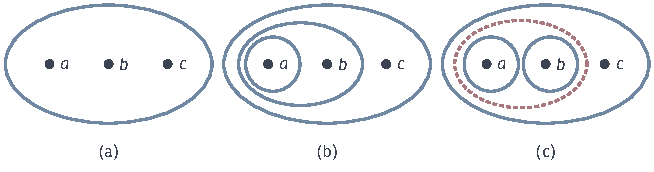
\includegraphics[width=110.786mm]{figures/04-spaces-measures-and-geometry/01-topology-and-metric/tikz/topo-finite-topologies/figure.pdf}
  \caption{三点集$X=\{a,b,c\}$上的三个子集族，每条蓝色闭曲线圈出族中的一个集合，空集未画出。(a)只有$X$，是拓扑。(b)$\{a\}$、$\{a,b\}$、$X$层层嵌套，是拓扑。(c)有$\{a\}$与$\{b\}$却缺少它们的并$\{a,b\}$（红色虚线），不是拓扑。}
  \label{fig:topo-finite-topologies}
\end{BookInlineFigure}

图(b)对应的族是
\[
 \mathcal T=\bigl\{\varnothing,\ \{a\},\ \{a,b\},\ X\bigr\}.
\]
它的成员依次包含，任取两个，并是较大的那个，交是较小的那个，结果都还在族中，所以$\mathcal T$是拓扑。图(c)的族含有$\{a\}$和$\{b\}$，它们的并$\{a,b\}$却不在族中，并封闭这一条不成立。

\paragraph{同一集合上的不同拓扑}
拓扑是附加在集合上的结构，同一个集合可以配上很不相同的拓扑。两个极端情形最能说明这一点。

\begin{example}[离散拓扑与平凡拓扑]
\label{ex:topo-discrete-indiscrete}
对任意集合$X$，全部子集组成的族$\mathcal P(X)$满足定义~\ref{def:topo-topology}，称为\term{离散拓扑}（discrete topology）。这时每个单点集$\{x\}$都是开集，$x$附近只有它自己。

另一端是$\{\varnothing,X\}$，它也满足三条规则，称为\term{平凡拓扑}（indiscrete topology）。这时唯一包含$x$的开集是整个$X$，空间中任何两点都无法用开集区分。

在两点集$X=\{a,b\}$上，$\{\varnothing,\{a\},X\}$也是拓扑。包含$b$的开集只有$X$，它也包含$a$；$a$却有一个不含$b$的开集$\{a\}$。在这个拓扑下，$a$总在$b$的每个开集里，反过来却不成立，“附近”这一关系可以不对称。
\end{example}

清单越长，可用来围住点的区域越多，点与点之间就越能区分。设$\mathcal T_1\subseteq\mathcal T_2$是同一集合上的两个拓扑，称$\mathcal T_2$比$\mathcal T_1$\term{更细}（finer），$\mathcal T_1$比$\mathcal T_2$更粗。

离散拓扑最细，平凡拓扑最粗，$\mathbb R$的通常拓扑介于二者之间。两个拓扑也可以互不包含：在$\{a,b\}$上，$\{\varnothing,\{a\},X\}$与$\{\varnothing,\{b\},X\}$就谈不上谁更细。

\subsection{拓扑基}
\label{sec:topo-basis}

实轴的开集可以形状复杂，例如$\bigcup_{n\geq1}(1/(n+1),1/n)$，但每个开集都是若干开区间的并：对开集$U$的每个点$x$取一个含于$U$的区间$(x-r_x,x+r_x)$，这些区间的并恰好是$U$。只要知道“开区间”这一小类集合，就能确定全部开集。

这与线性空间中用基表示向量相似：基向量通过线性组合得到所有向量，基本开集通过取并得到所有开集。类比到这里为止，因为取并没有系数，表示方式一般也不唯一，“基”的成员之间也不要求任何独立性。

\begin{definition}[拓扑基]
\label{def:topo-basis}
设$(X,\mathcal T)$是拓扑空间，$\mathcal B\subseteq\mathcal T$。若每个开集都能写成$\mathcal B$中若干成员的并，就称$\mathcal B$为$\mathcal T$的一个\term{拓扑基}（basis for a topology），$\mathcal B$的成员称为基本开集。
\end{definition}

空集是$\mathcal B$中零个成员的并，所以这一要求对空集自动成立。判断一个开集族是否为拓扑基时，逐点检验往往更方便：$\mathcal B\subseteq\mathcal T$是拓扑基，当且仅当对每个开集$U$和每个$x\in U$，都存在$B\in\mathcal B$使
\begin{equation}
 x\in B\subseteq U.
 \label{eq:topo-basis-pointwise}
\end{equation}

必要性是因为$x$属于表示$U$的某个成员。充分性是因为把这些$B$对$x\in U$取并，得到的集合含于$U$，又包含$U$的每个点，所以恰好等于$U$。图~\ref{fig:topo-basis-criterion}(a)画的就是这个判据：靠近边缘的点只是需要更小的基本开集。

\paragraph{由一族集合生成拓扑}
在欧氏空间里，我们往往先想到一类形状简单的集合，再希望用它们生成拓扑。这时需要判断：一族子集在什么条件下能作为某个拓扑的基。

\begin{theorem}[生成拓扑的基]
\label{thm:topo-basis-criterion}
设$X$是集合，$\mathcal B$是$X$的一族子集，满足
\begin{enumerate}
  \item $\mathcal B$的成员覆盖$X$，即每个$x\in X$都属于某个$B\in\mathcal B$；
  \item 若$x\in B_1\cap B_2$，$B_1,B_2\in\mathcal B$，则存在$B_3\in\mathcal B$使$x\in B_3\subseteq B_1\cap B_2$。
\end{enumerate}
令$\mathcal T$为$\mathcal B$中成员的所有并组成的族，则$\mathcal T$是$X$上的拓扑，$\mathcal B$是它的拓扑基。反过来，任何拓扑的拓扑基都满足这两条。
\end{theorem}
\begin{proof}
空集是零个成员的并，由条件1，$X$是全部成员的并，所以$\varnothing,X\in\mathcal T$。若干个“$\mathcal B$中成员的并”再取并，仍是$\mathcal B$中成员的并，所以$\mathcal T$对任意并封闭。

剩下验证两个集合的交。设$U=\bigcup_iB_i$，$V=\bigcup_jB'_j$，$x\in U\cap V$。则存在一对$i,j$使$x\in B_i\cap B'_j$，由条件2可取$B_x\in\mathcal B$，使
\[
 x\in B_x\subseteq B_i\cap B'_j\subseteq U\cap V.
\]
对$x\in U\cap V$取并，得到
\[
 U\cap V=\bigcup_{x\in U\cap V}B_x\in\mathcal T.
\]

反过来，设$\mathcal B$是拓扑$\mathcal T$的基。$X$是开集，必是$\mathcal B$中成员的并，条件1成立。$B_1\cap B_2$是开集，把判据\eqref{eq:topo-basis-pointwise}用于它，就得到条件2。
\end{proof}

条件2的作用可以从图~\ref{fig:topo-basis-criterion}(b)看出：两个基本开集的交不必本身是基本开集，但在交的每个点处都要放得下一个基本开集。

\begin{BookInlineFigure}
  \centering
  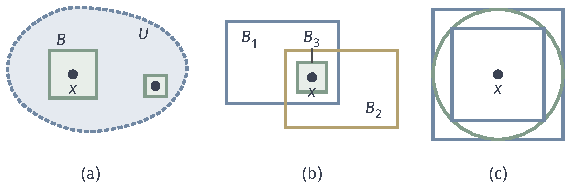
\includegraphics[width=96.227mm]{figures/04-spaces-measures-and-geometry/01-topology-and-metric/tikz/topo-basis-criterion/figure.pdf}
  \caption{拓扑基的三个判断。(a)开集$U$（虚线边界）中的每个点都有一个含于$U$的基本开集（绿色），靠近边界的点需要更小的方块。(b)定理条件2：在$B_1\cap B_2$的点$x$处放得下基本开集$B_3$。(c)以$x$为中心，正方形、圆盘、更小的正方形依次嵌套，所以方块与圆盘生成同样的开集。}
  \label{fig:topo-basis-criterion}
\end{BookInlineFigure}

条件2不能省略。在$X=\{a,b,c\}$上取$\mathcal B=\{\{a,b\},\{b,c\}\}$，它覆盖$X$。两个成员的交是$\{b\}$，而$\mathcal B$中没有成员能放进$\{b\}$，条件2不成立。所有的并组成的族是
\[
 \bigl\{\varnothing,\ \{a,b\},\ \{b,c\},\ X\bigr\},
\]
它不含$\{a,b\}\cap\{b,c\}=\{b\}$，的确不是拓扑。

\begin{example}[开区间与开矩形]
\label{ex:topo-intervals-rectangles}
全体开区间$(a,b)$构成$\mathbb R$通常拓扑的基，这正是本小节开头的观察。

在平面$\mathbb R^2$上，取全体开矩形$(a_1,b_1)\times(a_2,b_2)$组成的族$\mathcal B$。它覆盖$\mathbb R^2$，两个开矩形的交为
\[
\begin{aligned}
&\bigl((a_1,b_1)\times(a_2,b_2)\bigr)\cap\bigl((c_1,d_1)\times(c_2,d_2)\bigr)\\
&\qquad=\bigl((a_1,b_1)\cap(c_1,d_1)\bigr)\times\bigl((a_2,b_2)\cap(c_2,d_2)\bigr).
\end{aligned}
\]
两个开区间的交是开区间或空集，所以这个交仍是开矩形或空集，条件2成立。

由定理~\ref{thm:topo-basis-criterion}，开矩形生成$\mathbb R^2$上的一个拓扑，称为$\mathbb R^2$的通常拓扑。$\mathbb R^n$上用$n$个开区间的乘积同样处理。
\end{example}

不同的基可以生成同一个拓扑。在$\mathbb R^2$上改用全体开圆盘作基，条件1、2同样成立。如图~\ref{fig:topo-basis-criterion}(c)，圆盘内任一点周围都能放进一个以它为中心的小正方形，正方形内任一点周围也能放进一个小圆盘。由判据\eqref{eq:topo-basis-pointwise}，两族集合生成的开集完全相同，开集并不取决于用正方形还是圆形去度量附近。

\subsection{邻域}
\label{sec:topo-neighborhoods}

讨论一个点附近的性质时，用到的区域不必恰好是开集。要说“$f$在$x=1/2$附近取正值”，说它在$[0,1]$上取正值就够了，尽管$[0,1]$不是开集。关键在于这个集合包含一个围住$1/2$的开集。

\begin{definition}[邻域]
\label{def:topo-neighborhood}
设$X$是拓扑空间，$x\in X$。若集合$N\subseteq X$包含某个开集$U$，且$x\in U$，就称$N$是$x$的\term{邻域}（neighborhood）。本身是开集的邻域称为\term{开邻域}（open neighborhood）。
\end{definition}

在$\mathbb R$中，$[0,1]$是$1/2$的邻域，因为它包含开集$(1/4,3/4)\ni1/2$。它不是$0$的邻域，因为包含$0$的任何开集都含有负数，见图~\ref{fig:topo-neighborhoods}(a)。这说明两点：邻域本身不必是开集；“是邻域”总是相对于某个指定点而言，同一个集合可以是某些点的邻域而不是另一些点的邻域。

\begin{BookInlineFigure}
  \centering
  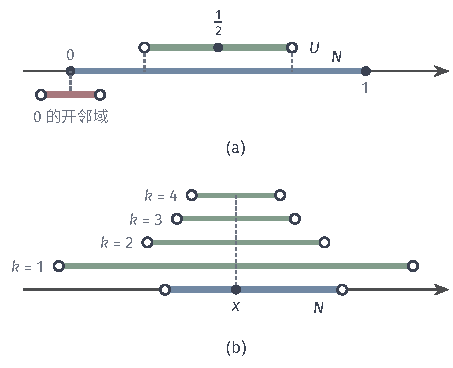
\includegraphics[width=76.793mm]{figures/04-spaces-measures-and-geometry/01-topology-and-metric/tikz/topo-neighborhoods/figure.pdf}
  \caption{邻域与邻域基。(a)蓝色的$N=[0,1]$包含绿色开集$U=(1/4,3/4)$，因此是$1/2$的邻域；$0$的任一开邻域（红色）都伸出$N$之外，所以$N$不是$0$的邻域。(b)绿色区间是$(x-1/k,x+1/k)$，蓝色区间是邻域$N=(x-0.4,x+0.6)$；$k=3$的区间已经含于$N$。}
  \label{fig:topo-neighborhoods}
\end{BookInlineFigure}

邻域与开集的关系可以反过来刻画开集：开集正是“对自己的每个点都是邻域”的集合。

\begin{lemma}[开集的邻域刻画]
\label{lem:topo-open-iff-neighborhood}
集合$U\subseteq X$是开集，当且仅当$U$是它的每个点的邻域。
\end{lemma}
\begin{proof}
若$U$开，对每个$x\in U$，$U$本身就是含$x$且含于$U$的开集。

反过来，若对每个$x\in U$都有开集$U_x$满足$x\in U_x\subseteq U$，则
\[
 U=\bigcup_{x\in U}U_x.
\]
拓扑对任意并封闭，所以$U$是开集。
\end{proof}

实轴开集的原始定义“每点两侧留有余地”正是这个引理的特例。以后证明一个集合是开集，常用的办法就是逐点找到含于其中的开邻域。

\subsection{邻域基}
\label{sec:topo-neighborhood-basis}

判断实数列$x_n\to x$时，并不需要检验$x$的所有邻域，只需检验区间$(x-1/k,x+1/k)$，$k=1,2,\dots$，因为任何邻域都包含其中某一个。这类足以代表所有邻域的子族，是描述一个点附近最经济的工具。

\begin{definition}[邻域基]
\label{def:topo-neighborhood-basis}
设$x\in X$，$\mathcal B_x$是$x$的一族邻域。若$x$的每个邻域$N$都包含$\mathcal B_x$中的某个成员，就称$\mathcal B_x$是$x$的\term{邻域基}（neighborhood basis）。
\end{definition}

在$\mathbb R$中，$\{(x-1/k,x+1/k):k\geq1\}$是$x$的邻域基。给定$x$的邻域$N$，它包含某个开集$U\ni x$，而$U$又包含某个$(x-r,x+r)$。取$k>1/r$，就有
\[
 \Bigl(x-\frac1k,x+\frac1k\Bigr)\subseteq(x-r,x+r)\subseteq N.
\]

图~\ref{fig:topo-neighborhoods}(b)是一个具体的情形：$N=(x-0.4,x+0.6)$的左侧余量是$0.4$，右侧余量是$0.6$，可取$r=0.4$。$k=2$时半径$0.5$超过左侧余量，$k=3$时半径$1/3<0.4$，区间已经含于$N$，更大的$k$也都一样。

闭区间族$\{[x-1/k,x+1/k]\}$同样是邻域基，所以邻域基的成员不必是开集。

\paragraph{邻域基与拓扑基的区别}
拓扑基与邻域基都是“用少数集合代表多数集合”，代表的对象却不同。拓扑基针对整个空间，用并生成每一个开集；邻域基只针对一个固定点，要求能塞进该点的每个邻域，并不生成任何开集。二者可以相互得到。

\begin{lemma}[由拓扑基得到邻域基]
\label{lem:topo-basis-to-neighborhood-basis}
若$\mathcal B$是$X$的拓扑基，则对每个$x\in X$，$\mathcal B_x=\{B\in\mathcal B:x\in B\}$是$x$的邻域基。反过来，若对每个$x$都选定一个由开集组成的邻域基$\mathcal B_x$，则$\bigcup_{x\in X}\mathcal B_x$是$X$的拓扑基。
\end{lemma}
\begin{proof}
设$N$是$x$的邻域，取开集$U$使$x\in U\subseteq N$。由判据\eqref{eq:topo-basis-pointwise}，有$B\in\mathcal B$使$x\in B\subseteq U$。这个$B$属于$\mathcal B_x$，且含于$N$。

反过来，设$U$开，$x\in U$。$U$是$x$的邻域，含有某个$B\in\mathcal B_x$，而$B$是开集且$x\in B$。于是$\bigcup_x\mathcal B_x$满足判据\eqref{eq:topo-basis-pointwise}。
\end{proof}

例如，$\mathbb R$的开区间基中包含$x$的那些区间构成$x$的邻域基，但它比$\{(x-1/k,x+1/k)\}$大得多：后者只用可数个集合就完成了同样的任务。一个点是否总有这样可数的邻域基，是第~\ref{sec:topo-countability}小节要讨论的问题。
